\documentclass[letter,11pt]{article}
\usepackage[spanish, activeacute]{babel}
\usepackage{amsfonts}
\usepackage{amsmath,amsfonts,amssymb}
\usepackage{fancyhdr}
\usepackage{fancyvrb}
\usepackage{xy}
\usepackage{graphicx}
\usepackage{latexsym,amsfonts}
\usepackage{enumerate}
\usepackage[spanish,activeacute]{babel}
\usepackage{multirow}
\usepackage{multicol}
\usepackage{hyperref}
\usepackage{longtable}


\textwidth 160mm
\textheight 235mm
\oddsidemargin 0.7cm
\topmargin -1cm

\usepackage[numbered,framed]{matlab-prettifier}
\lstMakeShortInline"
\lstset{
  style              = Matlab-editor,
  %basicstyle         = \mlttfamily,
  escapechar         = ",
  mlshowsectionrules = true,
  morekeywords={endif,endfor,endwhile},
}

\setlength{\oddsidemargin}{-0.5cm}
\setlength{\evensidemargin}{0cm} \setlength{\textwidth}{17.5cm}
\setlength{\textheight}{24cm} \setlength{\topmargin}{-1.7cm}
\newcommand{\N}{\mathbb{N}}

\title{lab02 521230 2018-1}

\addtolength{\voffset}{-1cm}

%\pagestyle{empty}

\parindent 0cm

\font\bff=cmbx10 at 10truept
\font\lg=cmdunh10 at 10truept
\font\bl=cmss10 at 10truept

\newcommand\R{\mathbb{R}}
\newcommand\IN{\mathbb{N}}
\newcommand\Z{\mathbb{Z}}
\newcommand\bsi{{\mbox{\boldmath $\sigma$}}}
\newcommand\bta{{\mbox{\boldmath $\tau$}}}
\newcommand\bet{{\mbox{\boldmath $\eta$}}}
\newcommand\bga{{\mbox{\boldmath $\gamma$}}}
\newcommand\bze{{\mbox{\boldmath $\zeta$}}}
\newcommand{\dis}{\displaystyle}

\renewcommand\u{\mathbf{u}}
\newcommand\bv{\mathbf{v}}
\newcommand\0{\mathbf{0}}

\newcommand\I{\mathbf{I}}
\def\e{\mathbf{e}}
\def\qen{{\quad\hbox{en}\quad}}
\newcommand\f{\mathbf{f}}
\newcommand\disp{\displaystyle}
\newcommand\bdiv{\mathbf{div}\,}
\newcommand\bnu{{\mbox{\boldmath $\nu$}}}
\renewcommand\div{\mathrm{div}\,}
\newcommand\tr{\mathrm{tr}\,}
\newcommand{\matlab}{{\sc Matlab}}
\newcommand{\octave}{{\sc Octave }}

\newcommand{\header}{
{\lg UNIVERSIDAD DE CONCEPCION}\hfill
\vskip-4truept
{\bff FACULTAD DE CIENCIAS}\hfill
\vskip-4truept
{\bff FISICAS Y MATEMATICAS}\hfill
\vskip-4truept
{\bl DEPARTAMENTO DE INGENIERIA MATEMATICA}\hfill
\vskip4truept\hrule\hrule\vskip4truept
\par
}

\begin{document}
\header
\vspace{0.7cm}
\begin{center}
\textbf{\small C\'alculo Num\'erico (521230) - Laboratorio 2}\\
\vspace{0.1cm}
\textbf{\Large INTRODUCCION A OCTAVE II}
\vspace{0.7cm}
\end{center}



%\bigskip
\section{Programas en \octave}
\medskip

Un programa inform\'atico es un conjunto de instrucciones (comandos) escritas en un determinado
lenguaje de programaci\'on. \octave incorpora muchos comandos para la soluci\'on de varios problemas matem\'aticos. En el Laboratorio 1 vimos, por ejemplo, el comando \Verb+norm+ para el c\'alculo de normas
de vectores y matrices. Otro ejemplo es \Verb+roots+, que permite calcular las ra\'{\i}ces de un polinomio
de grado $n \ge 1$.

Si escribimos en la ventana de comandos

\medskip
\begin{lstlisting}		
>> help roots
\end{lstlisting}
\medskip

\octave escribe un texto de ayuda para esta funci\'on. De acuerdo con esta ayuda, si queremos calcular las ra\'{\i}ces del polinomio $x^2 + 5x + 6$ con ayuda de la funci\'on \Verb+roots+, debemos darle como entrada un vector que contenga los coeficientes del polinomio. As\'{\i}, con la instrucci\'on

\medskip
\begin{lstlisting}		
>> roots([1 5 6])       % calcular raices de polinomio de grado 2
\end{lstlisting}
\medskip

\octave calcular\'a aproximaciones a las ra\'{\i}ces de $x^2 + 5x + 6$. Como no guardamos la salida de la funci\'on en ninguna variable, las ra\'{\i}ces del polinomio quedan guardadas en \Verb+ans+.

Si escribimos

\medskip
\begin{lstlisting}		
>> x = roots([1 0 -1])   % calcular raices de polinomio de grado 2
\end{lstlisting}
\medskip

\octave calcular\'a aproximaciones a las ra\'{\i}ces del polinomio $x^2-1$,
las cuales no quedar\'an guardadas en \Verb+ans+, sino en \Verb+x+.

Con este ejemplo hemos visto algunos detalles importantes de programas en \octave:

\begin{enumerate}			
\item Todos los programas deben ser escritos en el editor de \octave, el cual se muestra en la Figura \ref{fig:editor}. Para abrir el editor, en la ventana primcipal de \octave{} hacer click en \emph{New Script} (el primer bot\'on en la esquina superior izquierda) o apretar el atajo del teclado \verb"Cntrl+4". 

\begin{figure}[h]
\centering
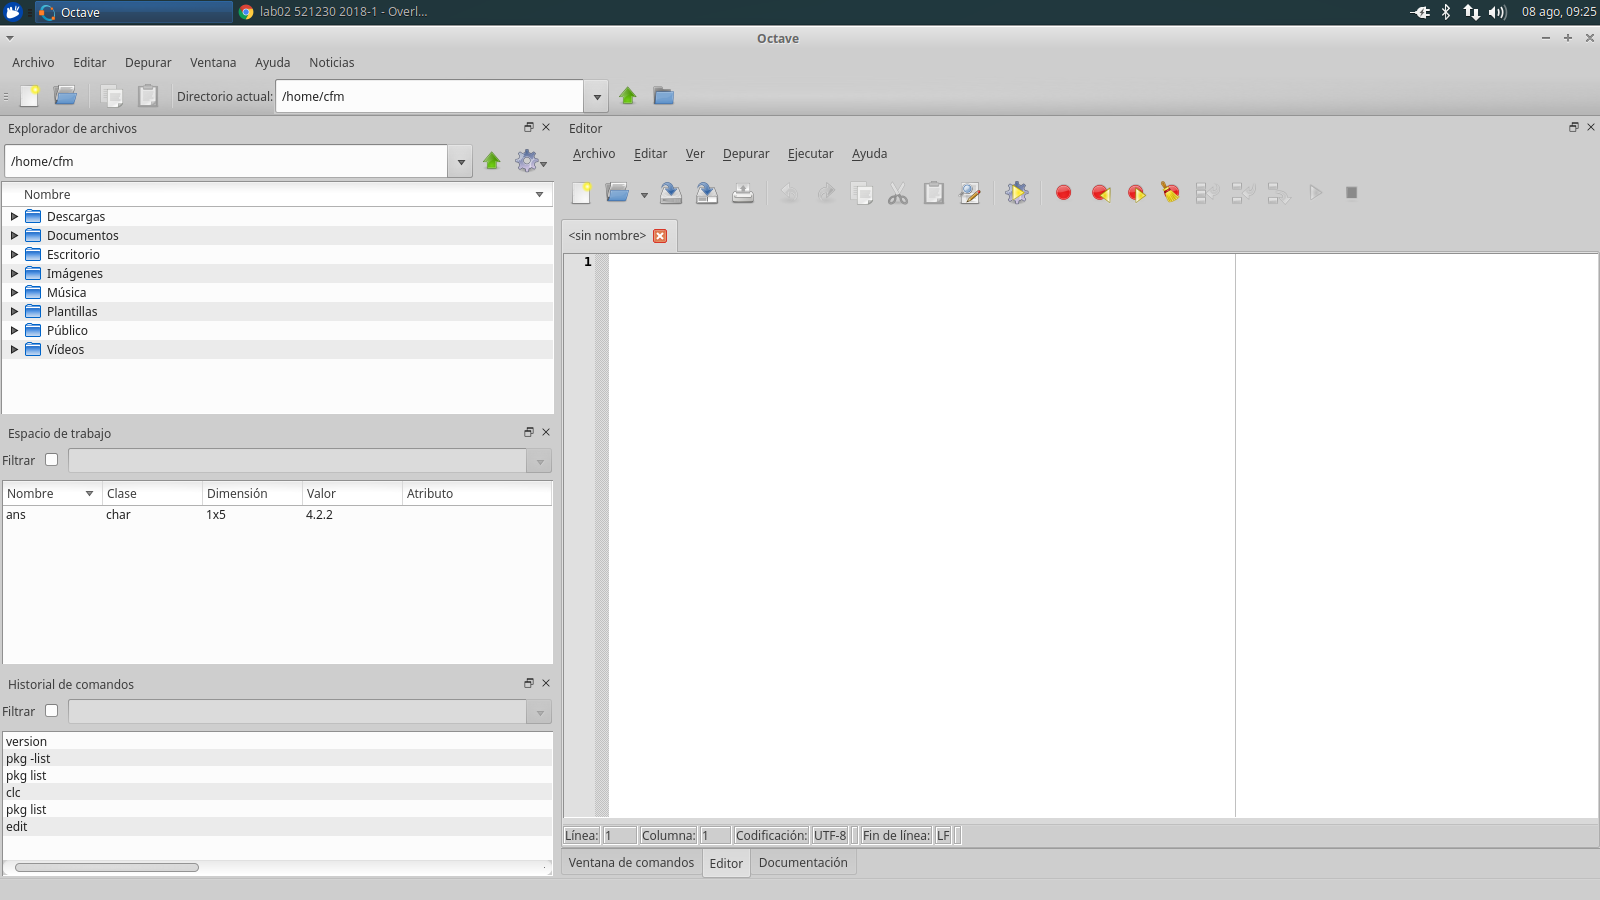
\includegraphics[width=0.8\textwidth]{editor_octave.png}
\caption{Editor de \octave.}\label{fig:editor}
\end{figure}

\item Todos los programas \octave deben guardarse en archivos con extensi\'on \Verb+.m+. Para ello, en la ventana del editor haga click en el \'icono \emph{Save File} (el tercer bot\'on a la izquierda), y luego seleccione el directorio donde guardar\'a su archivo.

\item Un programa debe ser ejecutado desde la ventana de comandos.

Al llamar a un programa desde la ventana de comandos, \octave buscar\'a el archivo con nombre igual al programa y extensi\'on \Verb+.m+ en sus directorios de b\'usqueda. Con el comando \Verb+path+ podremos ver cuales son estos directorios, con \Verb+addpath, rmpath+ podremos modificarlo.

Evidentemente, en el \verb"path" por defecto, \octave{} tiene guardados los programas y comandos que trae incorporado. \index{path}\index{addpath}\index{rmpath}

Si el programa no se encuentra en el directorio de b\'usqueda, \octave lo buscar\'a en el directorio de trabajo actual, el cual se puede ver en la barra superior de la ventana principal de \octave. En estas ventanas podemos cambiar y navegar por los directorios (tambi\'en podemos verlos y cambiarlos con \Verb+cd+)\index{cd}.

\item Una vez encontrado el archivo y si lo hemos llamado de manera correcta, \octave ejecutar\'a las insctrucciones en \'el.
Note que si en la ventana de comandos de \octave  escribimos

\medskip
\begin{lstlisting}		
>> x = roots(1 0 -1)
\end{lstlisting}
\medskip

\noindent \octave no podr\'a calcular las ra\'{\i}ces del polinomio $x^2 -1$, pues no hemos llamado al programa de manera correcta.

\item En un programa, todo lo que siga al s\'{\i}mbolo \Verb+%+ 
es interpretado como un comentario y los primeros comentarios que se escriban constituyen una ayuda al programa y se mostrar\'an cuando en la ventana de comandos se escriba

\Verb+help <nombre del programa>+.

\item Existen dos tipos de programas en \octave: ruteros y funciones. 

Una funci\'on permite par\'ametros de entrada y salida, un rutero no (m\'as a\'un, el rutero es una ``recopilaci\'on''  ordenada de comandos que pueden ser ejecutados con una sola en la ventana de comandos). La primera l\'{\i}nea del programa en una funci\'on tiene que ser de la forma

\Verb+function [salida] = <nombre funcion>(entrada)+

\noindent \Verb+salida+ es una lista con los nombres de los par\'ametros de salida de la funci\'on separados por comas, mientras que \Verb+entrada+ es una lista con los nombres de todos los par\'ametros de entrada a la funci\'on tambi\'en separados por comas.			

\textbf{Obs. 1:} Una diferencia importante entre funciones y ruteros es que las variables que se usen en una funci\'on son locales a la funci\'on, mientras que las que se usen en un rutero son globales, es decir, seguir\'an existiendo una vez que termine la ejecuci\'on del programa.	

\textbf{Obs. 2:} Una forma directa de crear una funci\'on desde la ventana principal de \octave{} es hacer click en \verb"File>New" y luego en \emph{Function}.

\textbf{Obs. 3:} Un programa tipo rutero puede ser  ejecutado desde el editor haciendo click en el bot\'on \emph{Save File and Run}, ubicado en el centro de la ventana del editor. Observe que alrededor de ese bot\'on aparecen otras opciones de ejecuci\'on m\'as avanzadas (que no se ver\'an en este curso). 

\end{enumerate}	

\section{\octave y sus funciones}
  La versatilidad de \octave se basa en sus funciones. En particular, la funci\'on \texttt{help} es muy importante. Esta funci\'on nos permite leer un resumen del uso de otras funciones. Por ejemplo, si ejecutamos 
  \begin{lstlisting}
   help abs
  \end{lstlisting}
  obtendremos una salida como
  \begin{lstlisting}
    abs    Absolute value.
    abs(X) is the absolute value of the elements of X. When
    X is complex, abs(X) is the complex modulus (magnitude) of
    the elements of X.
  \end{lstlisting}
  Mediante una breve lectura observamos que la funci\'on \texttt{abs()} nos permite obtener el valor absoluto de los elementos de una matriz. Entre las principales funciones de \octave cuentan:
  \begin{center}
      \begin{tabular}{p{5cm}|l}
        \hline
	Sentencia	  & Significado\\
	\hline
       abs()		  & Valor absoluto\\
       cos(),sin(),tan()  & Funciones trigonom\'etricas en radianes\\
       if()		& Verificador l\'ogico\\
       plot()		& Permite dibujar figuras planas\\
       ones()		& Crea una matriz con todas las entradas en 1\\
       zeros()		& Crea una matriz con entradas todas nulas \\
       find()		& Encuentra los \'indices de una matriz que son no nulos\\
       disp()		& Muestra una cadena\footnote{Ver siguiente secci\'on} en la ventana de comando\\
       input()		& Recibe una variable a trav\'es del teclado del ordenador\\
       norm() 		& Norma Euclideana de un vector \\
       cross()		& Producto cruz de vectores \\
       dot()		& Producto interior o punto de vectores
      \end{tabular}
  \end{center}

Utilice la funci\'on \texttt{help()} para conocer los distintos funcionamientos de cada una de estas funciones.

 \section{Ciclos y condicionales en \octave}

\begin{enumerate}
\item Ciclo \Verb+for+: tiene la forma

\medskip

\begin{lstlisting}		
for var = vi:incr:vf
<instrucciones>
endfor
\end{lstlisting}

\medskip

\noindent Las instrucciones en el cuerpo de este ciclo se ejecutan
tantas veces como valores tome la variable \Verb+var+, la que
se inicializa con \Verb+vi+ y toma los valores
\Verb@vi@, \Verb@vi+incr@, \Verb@vi+incr+incr@, ..., \Verb@vf@.
Si \Verb+incr+ es 1, puede escribirse

\medskip

\begin{lstlisting}		
for var = vi:vf
<instrucciones>
endfor
\end{lstlisting}

\medskip

\noindent Si, queremos, por ejemplo, sumar los $10$ primeros n\'umeros
naturales con ayuda de un ciclo \Verb+for+ deber\'{\i}amos
escribir\index{for}

\medskip

\begin{lstlisting}
suma = 0
for i = 1:10
suma = suma + i
endfor
\end{lstlisting}

\medskip

\noindent Si, queremos, por ejemplo, guardar en un vector \verb+p+ los
10 primeros t\'erminos de la progresi\'on geom\'etrica (con primer t\'ermino
igual a 1 y raz\'on igual a 3)
\[
1,\,3,\,9,\,27,\,81,\,\cdots
\]
podr\'{\i}amos hacerlo con ayuda de un ciclo \verb+for+ de la siguiente manera

\medskip

\begin{lstlisting}
p = zeros(10,1);    % inicializar p
p(1) = 1;           % primer elemento de p es 1
for i = 2:10
p(i) = 3*p(i-1);
endfor
\end{lstlisting}

\medskip

\item Ciclo \Verb+while+: tiene la forma

\medskip

\begin{lstlisting}		
while <condicion>
<instrucciones>
endwhile
\end{lstlisting}

\medskip

\noindent Las instrucciones en el cuerpo del ciclo se ejecutan mientras
\Verb+condicion+ sea verdadera.

% 				\noindent Si, queremos, por ejemplo, sumar los $10$ primeros n\'umeros
% 				naturales con ayuda de un ciclo \Verb+while+ deber\'{\i}amos
% 				escribir\index{while}
%
% 				\medskip
%
% 				\begin{lstlisting}[gobble=4,frame=none]
% 					suma = 0
% 					i = 1
% 					while i <= 10
% 					   suma = suma + i
% 					   i = i + 1
% 					end
% 				\end{lstlisting}
% 				
% 				\medskip

\noindent El vector \verb+p+ del ejemplo anterior tambi\'en puede crearse con un ciclo \verb+while+
de la siguiente forma:

\medskip

\begin{lstlisting}
p = zeros(10,1);    % inicializar p
p(1) = 1;           % primer elemento de p es 1
i = 2;
while i <= 10
p(i) = 3*p(i-1);
i = i + 1;
endwhile
\end{lstlisting}

\medskip

%\newpage	
\item Una condicional en \octave\, tiene la forma general

\medskip

\begin{lstlisting}		
if <condicion>
<instrucciones 1>
[elseif
<instrucciones 2>
else
<instrucciones 3>]
endif			
\end{lstlisting}				

\medskip

\noindent donde \Verb+condicion+ es una expresi\'on l\'ogica e
\Verb+instrucciones+ es el conjunto de comandos que se
ejecutar\'a si \Verb+condicion+ es verdadera. Los comandos encerrados
entre corchetes son opcionales.\index{condicional}

\end{enumerate}	

\textbf{Ejemplo 1.}

Abramos un archivo nuevo en el editor de \octave. En el primero escribamos las instrucciones siguientes:
	
    \medskip

\begin{lstlisting}		
function F = mifuncion1(x)
% funci\'on para evaluar f(x) = (1-cos(x))/x^2 (si x~=0) 
% y f(0) = 1/2 en cada una de las componentes del vector de entrada v

% creando vector de ceros con mismo n\'umero de elementos que x
F = zeros(length(x),1);

% ciclo para evaluar f en componentes de x
for i=1:length(x)
% averiguar si componente i-esima de v es distinta de cero
if x(i) ~= 0
F(i) = (1-cos(x(i)))/x(i)^2;
else
F(i) = 1/2
endif
endfor
\end{lstlisting}

\medskip

Esta es la funci\'on que permite evaluar una funci\'on $f$.	Guardemos este programa en \Verb+/home/cfm/mifuncion1.m+.
\smallskip

{\bf Observaci\'on:} El nombre del archivo donde guardamos la funci\'on
y el nombre de la funci\'on (en 1ra l\'{\i}nea del programa) coinciden.
Durante todo el semestre mantendremos esta convenci\'on.	

\smallskip

Regresemos a la ventana de comandos de \octave\, para llamar a \Verb+mifuncion1+.
Si queremos, por ejemplo, averiguar los valores de $f$ en \verb"0, 0.1, 0.2, 0.3, 0.4, 0.5", podemos hacerlo mediante

\medskip

\begin{lstlisting}
>> mifuncion1(0:.1:.5 )   % evaluar f en [0,0.1,0.2,0.3,0.4,0.5]
>> whos                   % ni x ni F (locales a mifuncion1) aparecen
% como variables de memoria
\end{lstlisting}

\medskip

Evaluemos $f(x)$ en los puntos $0.188 \times 10^{-7}$, $0.189\times 10^{-7}$, $0.19\times 10^{-7}$
llamando a \Verb+mifuncion1+

\medskip

\begin{lstlisting}		
>> mifuncion1([0.188e-7, 0.189e-7, 0.19e-7])
\end{lstlisting}

\medskip

Observe que los valores que retorna \Verb+mifuncion1.m+ son todos mayores que
$0.6$.

\begin{description}
\item[\textbf{Ejemplo 2.}] Escriba un rutero para graficar a la funci\'on $f$ en \eqref{ejemplo1}
en 100 puntos equidistantes en $[-\pi,\,\pi]$.
\end{description}

	Abramos un archivo nuevo, y es\-cri\-ba\-mos:
	
    \medskip

\begin{lstlisting}
% rutero para graficar f(x) = (1-cos(x))/x^2 entre -pi y pi
x = linspace(-pi,pi);
Fx = mifuncion1(x);
% grafiquemos la funci\'on
plot(x, Fx)
\end{lstlisting}

\medskip

y guard\'emoslo en el archivo \Verb+/home/cfm/plotmifuncion1.m+.	
\'Este es el rutero para graficar $f(x)$.
Si escribimos en la ventana de comandos

\medskip

\begin{lstlisting}		
>> help plotmifuncion1
\end{lstlisting}

\medskip

\octave\, muestra los primeros comentarios en \Verb+plotmifuncion1.m+.

Llamemos al rutero para ver el gr\'afico de $f(x)$
con $x \in [-\pi,\,\pi]$

\medskip

\begin{lstlisting}		
>> plotmifuncion1
>> whos              % las variables x y Fx permanecen en memoria
\end{lstlisting}

\medskip

Con el gr\'afico obtenido
nos damos cuenta de que la funci\'on parece ser siempre menor o igual que $\frac 1 2.$
Sin embargo, al evaluar $f$ en los puntos $0.188 \times 10^{-7}$, $0.189\times 10^{-7}$ y
$0.19\times 10^{-7}$ obtuvimos valores mayores que $0.5$.
\'Este es un ejemplo t\'{\i}pico de {\em cancelaci\'on excesiva}, la cual puede ocurrir
cuando se restan dos cantidades casi iguales. En la expresi\'on $(1-\cos(x))/x^2$
si $x \approx 0$, entonces $\cos(x) \approx 1$ y al hacer $1-\cos(x)$ se estar\'an restando dos
n\'umeros casi iguales.

\begin{description}
\item[\textbf{Ejemplo 3.}] Escriba una funci\'on que eval\'ue $e^x$ mediante su serie de Taylor $\displaystyle e^x=\sum_{n=0}^{\infty} \dfrac{x^n}{n!}$.
\end{description}

Abramos un archivo nuevo, es\-cri\-ba\-mos:

\medskip

\begin{lstlisting}			
function y=miexp(x)
y=1;
sum=x;
n=1;
while (y+sum~=y)
y=y+sum;
n=n+1;
sum=x*sum/n;
endwhile
\end{lstlisting}

\medskip

y guard\'emoslo en el archivo \Verb+/home/cfm/miexp.m+. Explique por qu\'e este programa siempre se detiene y compare los valores de esta funci\'on con los de la funci\'on de \octave  \texttt{exp(x)} para distintos valores de $x$.

\medskip
\textbf{Ejemplo 4.} 
Supongamos que deseamos tener un fichero que nos permita conocer el valor de las im\'agenes de la funci\'on 
$y=sin(x+x^2)$. Nos interesar\'ia que dado un valor para $x$ nos retorne el valor para $y$. En este caso podemos hacer:
\begin{verbatim}
 function y=f(x)
  y=sin(x+x.^2);
\end{verbatim}
observe que en tal caso la operaci\'on potenciaci\'on debe anteponerse con el operador \texttt{.} para que la 
potenciaci\'on sea componente a componente. Obviamente la entrada $x$ de esta funci\'on puede ser cualquier matriz, y 
la salida ser\'a una matriz de las mismas dimensiones.

Si nos interesara dibujar tal funci\'on en el intervalo $[-10,10]$, podemos hacer 
directamente
\begin{verbatim}
  x=[10:0.1:10];
  y=f(x);
  plot(x,y);
\end{verbatim}

Tambi\'en podemos definir funciones definidas por tramos usando este tipo de ficheros. Por ejemplo, si 
interesa ingresar a \octave la funci\'on 
$$
g(x):=\begin{cases}
       x^2+1 		&  x>0	\\
       \frac{1}{x^2+1} & x\leq 0
      \end{cases}
$$
podemos crear el fichero funci\'on
\begin{verbatim}
 function y=g(x)
    in=find(x>0);
    y(in)=x(in).^2+1;
    in=find(x<=0);
    y(in)=1./(x(in).^2+1);
\end{verbatim}

\section{Funciones como objetos inline}

Los objetos \texttt{inline} son otra forma de representar funciones en \octave. Por ejemplo, para 
crear un objeto inline que nos permita manejar la funci\'on $g(x)=33x^2+cos(e^x)$, debemos simplemente 
ejecutar la instrucci\'on
\begin{lstlisting}
g=inline('33*x.^2+cos(exp(x))','x');
\end{lstlisting}
Una vez creado este tipo de dato, podemos dibujarlo r\'apidamente haciendo uso de la funci\'on $\texttt{ezplot()}$, 
seg\'un
\begin{lstlisting}
 ezplot(g)
\end{lstlisting}
La primera cadena de las entradas de \texttt{inline()} es la forma vectorizada de la operaci\'on 
que define a la funci\'on, mientras que la segunda entrada y siguientes, especifican las variables 
que independientes de la funci\'on a definir.

\section{Arreglo de funciones}
  La instrucci\'on 
    \begin{lstlisting}
     arreglo=@nombre
    \end{lstlisting}
    retorna  un arreglo de funciones llamado \texttt{arreglo} que tiene 
    una funci\'on llamada \texttt{nombre}.
    
    Un arreglo de funci\'on es un objeto de \octave que permite llamar a funciones indirectamente. Se pueden utilizar para definir otras funciones e inclusive se pueden agrupar dentro de arreglos tipo celda.

    Cuando queramos definir una nueva funci\'on a trav\'es de un arreglo de funciones, utilizaremos funciones an\'onimas, que se generan como se ejemplifica a continuaci\'on. Supongamos que nos interesa ingresar a \octave la funci\'on de la par\'abolas $y=2x^2+3x+1$. Esto lo hacemos seg\'un
    \begin{lstlisting}
     a = 2;
     b = 3;
     c = 1;
     parabola = @(x) a*x.^2 + b*x + c;
    \end{lstlisting}
    Para poder dibujar este tipo de funciones hacemos uso de \texttt{plot()}.
    \begin{lstlisting}
    x=linspace(0,10,100);
    plot(x,parabola(x));
    \end{lstlisting}
    
    \section{La ventana gr\'afica}
      Como vimos en los ejemplos anteriores, sin importar el m\'etodo que usemos para graficar, \octave siempre crear\'a otra ventana, llamada por defecto \texttt{Figure 1}, similar a la Figura \ref{fig:ventanagrafica}. 
      \begin{figure}[htp]
      \begin{center}
      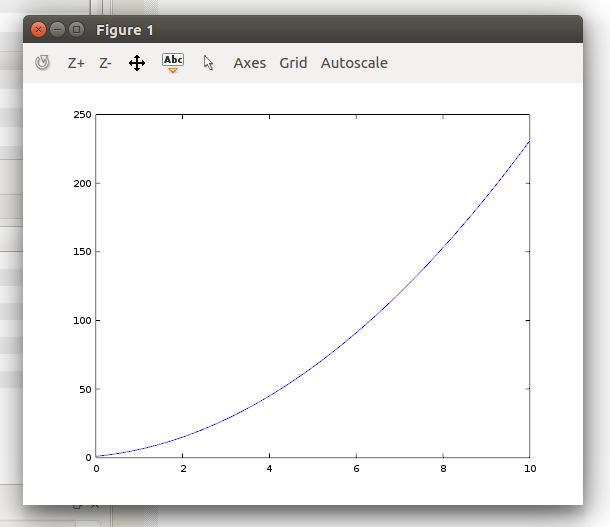
\includegraphics[width=0.4\textwidth]{./ventanafigure.png}
      \caption{\sl Ventana gr\'afica por defecto de \octave.}
      \label{fig:ventanagrafica}
      \end{center}
      \end{figure}
     Para crear una nueva ventana gr\'afica donde dibujar hacemos uso de la funci\'on \texttt{figure()}. Por 
     ejemplo, las intrucciones
     \begin{lstlisting}
      figure(1);
      ezplot(inline('x^2'));
      figure(2);
      ezplot(inline('x^2-1'));
      figure(3);
      ezplot(inline('x^2-2'));
     \end{lstlisting}
     crear\'an tres ventanas gr\'aficas llamadas \texttt{Figure 1, 2 } y \texttt{3}, las cuales se abrir\'an 
     en ese orden con tres gr\'aficas muy similares.
     Si nos interesa adjuntar estos tres gr\'aficos en una misma ventana gr\'afica hacemos uso del 
     comando \texttt{hold on}, como se ilustra a continuaci\'on,
     \begin{lstlisting}
     figure(4); hold on;
      ezplot(inline('x^2'));
      ezplot(inline('x^2-1'));
      ezplot(inline('x^2-2'));
     \end{lstlisting}
     si finalmente no deseamos agregar m\'as gr\'aficos a esta figura, ejecutamos 
     \begin{verbatim}
      hold off;
     \end{verbatim}  
     Si se desea que las gr\'aficas adjuntas cambien de colores autom\'aticamente se puede usar la instrucci\'on \texttt{hold all;} en vez de \texttt{hold on;}.
     
     Adem\'as, como anotaciones podemos agregar texto en ciertos lugares de los gr\'aficos de una figura. Mientras 
     la figura en la que deseamos a\~nadir un comentario est\'e seleccionada con el comando \texttt{figure()}, ejecutamos el 
     comando \texttt{gtext()}. Si conocemos la coordenada exacta donde queremos hacer un comentario, podemos 
     utilizar la funci\'on \texttt{text()}.
     
     \subsection{Opciones de estilo en gr\'aficos}
     
     A modo de ejemplo, a continuaci\'on presentamos un c\'odigo que sobrepone aproximaciones 
     en serie de Taylor de la funci\'on $y=sen(x)$ y formatea un gr\'afico con varios detalles.
     Para acceder al rutero ingrese a 
     \url{http://www.udec.cl/~fmilanese/codigo4.txt}.
      L\'ealo y ejec\'utelo en un rutero.
      
      \subsection{Opciones de estilo para dibujar curvas en 2D}

      Las opciones de estilo del comando \texttt{plot()} son una cadena que consiste en hasta tres 
      caracteres que especifican color, el estilo de l\'inea y forma de marcar los puntos de una gr\'afica.
      Estos caracteres son resumidos en la siguiente tabla
      
      \begin{center}
      \begin{tabular}{|c|c|c|}
Estilo de color & Estilo de linea & Estilo de marcador 	\\
\hline
\begin{tabular}{p{5mm}c}
 y & amarillo 	\\
 m & magenta  	\\
 r & rojo 	\\
 g & verde	\\
 b & azul	\\
 w & blanco	\\
 k & negro
\end{tabular}
&
\begin{tabular}{p{5mm}c}
 - & solida 	\\
-- & rayada  	\\
 : & punteada 	\\
-. & raya punto	\\
none & sin l\'inea \\
\end{tabular}
&
\begin{tabular}{p{5mm}c}
 + & signo de suma 	\\
 o & circulo  	\\
 * & asterisco 	\\
 x & con una equis	\\
 . & con un punto \\
$\wedge$ & tri\'angulo 	\\
 s & cuadrado 	\\
 d & diamante	\\
\end{tabular}
 \end{tabular}
 \end{center}
 
 los cuales puede ser usados como
 
 \begin{verbatim}
  plot(x,y,'r*')  %dibuja con linea roja continua y con marcadores asterisco
  plot(x,y,'b--') %dibuja con linea azul rayada
  plot(x,y,'+')   %dibuja puntos no conectados con un marcador +
 \end{verbatim}

 \section{Subgr\'aficas en una figura}

 Si se quiere hacer varios gr\'aficos dentro de una misma figura, pero 
 no sobreponerlos, se utiliza el comando \texttt{subplot()}. Este comando requiere tres 
 entradas de numeros enteros \texttt{subplot(m,n,p)} y representa dividir
 la ventana gr\'afica en $m\times n$ subventanas y elegir la subventana $p-$\'esima, 
 contadas por filas, como ventana de dibujo.
 
  Por ejemplo
  \begin{lstlisting}
   subplot(2,2,3)
  \end{lstlisting}
  dividir\'a la ventana gr\'afica actual en cuatro subventanas y dibujar\'a lo siguiente en la ventana 
  inferior izquierda.
 
  \section{Resumen de las principales funciones para graficar 2D}

 En la siguiente tabla se encuentran las principales funciones para hacer gr\'aficas 2D.

 \begin{center}
 \begin{tabular}{|p{2cm}|c||}
 Nombre				& Descripci\'on			\\
 \hline 
  \texttt{fplot()}		& Crea un gr\'afico de una funci\'on de una variable\\
  \texttt{bar()}		& Crea un gr\'afico de barras vertical\\
  \texttt{contour()}		& Crea un gr\'afico de curvas de nivel\\
  \texttt{contourf()}		& Crea un gr\'afico de curvas de nivel llenas\\
  \texttt{polar()}		& Dibuja curvas descritas en coordenadas polares\\
  \texttt{quiver()}		& Dibuja campos vectoriales\\
 \end{tabular}
 \end{center}
 
 a continuaci\'on ejemplos de usos de estos c\'odigos.
 
 \begin{center}
  \begin{longtable}{||l|c|c||}
   Funci\'on 		& C\'odigo 		& Salida \\
   \hline

\texttt{fplot()}		
  &
\begin{minipage}{3in}
\begin{verbatim}
f='sin(x.^2+3*x)'
fplot(f,[-10,pi])
\end{verbatim}

Notar que $f$ debe estar definida en $x$.
\end{minipage}
&
\begin{minipage}{0.3\textwidth}
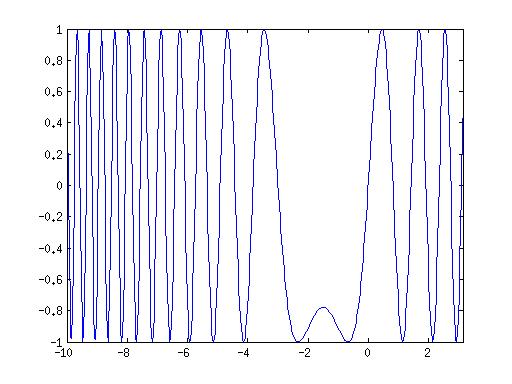
\includegraphics[width=\textwidth]{./ej1.jpg}
\end{minipage}
\\
\hline
\texttt{bar()}		
  & 
\begin{minipage}{3in}
\begin{verbatim}
t=linspace(0,2*pi,200);
r=sqrt(abs(2*sin(5*t))) ;
y=r.*sin(t);
bar(t,y);
axis([0 pi 0 inf ]);
\end{verbatim}
\end{minipage}
&
\begin{minipage}{0.3\textwidth}
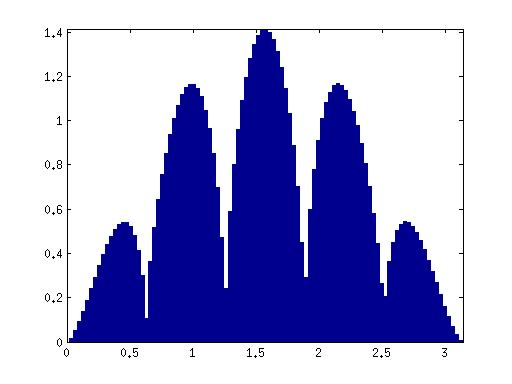
\includegraphics[width=\textwidth]{./ej2.jpg}
\end{minipage}
\\
\hline
  \texttt{contour()}		& 
\begin{minipage}{3in}
\begin{verbatim}
r =-5:.2:5;
[X,Y]=meshgrid(r,r) ;
Z=-.5*X.^2 +X.*Y+Y.^2;
cs=contour(X,Y,Z);
clabel(cs);
\end{verbatim}
\end{minipage} 
&
\begin{minipage}{0.3\textwidth}
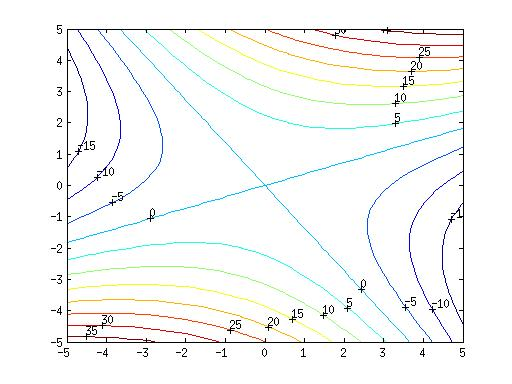
\includegraphics[width=\textwidth]{./ej3.jpg}
\end{minipage}
\\
\hline
  \texttt{polar()}		& 
\begin{minipage}{3in}
\begin{verbatim}
t=linspace(0,2*pi,200);
r=sqrt(abs(2*sin(5*t))) ;
polar(t,r);
\end{verbatim}
\end{minipage} 
&
\begin{minipage}{0.3\textwidth}
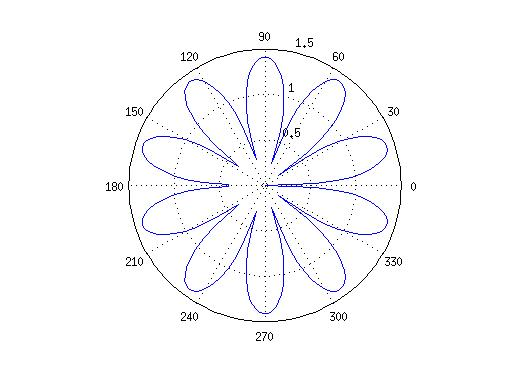
\includegraphics[width=\textwidth]{./ej4.jpg}
\end{minipage}
\\
\hline
  \texttt{quiver()}		& 
\begin{minipage}{3in}
\begin{verbatim}
r=-2:.2:2;
[X,Y]=meshgrid(r,r) ;
Z=X.^2-5*sin(X.*Y)+Y.^2;
[dx,dy]=gradient(Z,.2,.2);
quiver(X,Y,dx,dy,2);
\end{verbatim}
\end{minipage}
&
\begin{minipage}{0.3\textwidth}
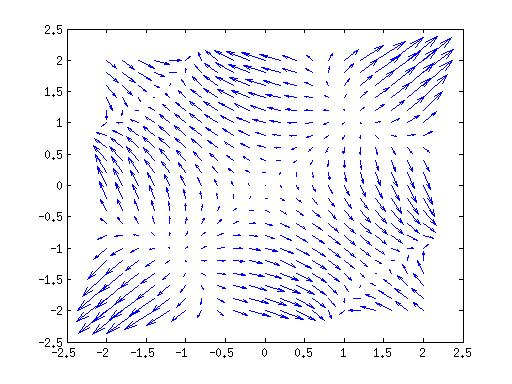
\includegraphics[width=\textwidth]{./ej5.jpg}
\end{minipage}
\\
  \end{longtable}
 \end{center}


\section{Errores comunes en \octave}
Los errores son una parte fundamental de nuestras vidas, interactuemos o no con \octave. La \'unica diferencia es que, cuando intereactuamos con ordenadores, se nos indican inmediatamente nuestros errores.

Hay que advertir que programar en \octave requiere de tiempo y concentraci\'on. Si no tenemos el tiempo o la concentraci\'on adecuada se puede volver muy irritante, si por un momento no hacemos la distinci\'on entre (, [ \'o \{, o simplemente no distinguimos entre : y ;, o nos olvidamos de considerar que \texttt{a} es distinto de \texttt{A}, entonces programar en \octave se volver\'a lento y tedioso.

A continuaci\'on se enlistan los errores mas comunes con los que nos encontraremos mientras trabajamos con \octave. Se adjuntan ejemplos de los errores y explicaciones de ellos.

\subsection{Indices de asignaci\'on no coinciden}
\begin{lstlisting}
>>  D=zeros(3); d=[1,2];
>> D(2:3,:)=d;
error: A(I,J,...) = X: dimensions mismatch
\end{lstlisting}
Este error sucede cuando hay asignaciones de matrices  y las matrices que est\'an a ambos lados del signo \texttt{=} no tienen la misma dimensi\'on. Utiliza el comando \texttt{size()} para 
chequear las dimensiones de ambos elementos y asegurarte que coincidan. En este 
ejemplo tendriamos que
\begin{lstlisting}
>> size(D(2:3,:))

ans =

2     3

>> size(d)

ans =

1     2
\end{lstlisting}

\subsection{Mal uso de (, [, \{}
\begin{lstlisting}
>> (x,y)=sphere(5)
parse error:

  syntax error

>>> (x,y)=sphere(5)
      ^
\end{lstlisting}
Aqu\'i lo que sucede es que \octave se confunde con las variables de salida de \texttt{sphere}. Al verlas dentro de par\'entesis \verb"( , )" ellas representan indices de una matriz y no variables. Las salidas de una  funci\'on  deben ser encerradas en par\'entesis \verb"[". 

Tambi\'en, cuando los par\'entesis no est\'an escritos correctamente, el mismo error es mostrado. Por ejemplo
\begin{lstlisting} 
>>  (x,y]=sphere(5)
parse error:

  syntax error

>>>  (x,y]=sphere(5)
       ^
\end{lstlisting}

\subsection{Errores de \'indice y dimensi\'on}
\begin{lstlisting}
>> x=1:100;
>> v=0:3:45;
>> s=x(v);
error: subscript indices must be either positive integers less than 2^31 or logicals
\end{lstlisting}
El primer elemento del vector de \'indices \texttt{v} es cero. En consecuencia, estamos 
intentando obtener el $0^{avo}$ elemento de \texttt{x}, pero cero no es un \'indice v\'alido  para un vector ni para una matriz. El mismo error sucede cuando un n\'umero negativo aparece  como \'indice. Adem\'as, cuando un \'indice excede el la dimensi\'on de una variable,  tambi\'en sucede un error, siguiendo el ejemplo anterior:
\begin{lstlisting}
>> x=1:100;
>> v=1:3:103;
>> s=x(v);
error: A(I): index out of bounds; value 103 out of bound 100
\end{lstlisting}
Los ejemplos aqu\'i ilustrados son casi triviales. La mayor\'ia de las veces, estos errores aparecen cuando los \'indices son creados, incrementados o manipulados dentro de un ciclo.

\subsection{Operaciones matriciales}
\begin{lstlisting}
>>  x=1:10; y=20:-2:1;
>> x*y
error: operator *: nonconformant arguments (op1 is 1x10, op2 is 1x10)
\end{lstlisting}
Cuando realizamos la multiplicaci\'on matricial \texttt{x*y}, el n\'umero de columnas 
de \texttt{x} debe coincidir con el n\'umero de filas de \texttt{y}. En el ejemplo anterior 
\texttt{x} e \texttt{y} son ambos vectores de tama\~no $1\times 10$, por lo tanto 
no se pueden multiplicar. Sin embargo, \texttt{x*y'} y \texttt{x'*y} si se puede ejecutar, 
los que representan los productos exterior (cruz) e interior (punto) del vector \texttt{x} con el 
vector \texttt{y}.

Muchas otras operaciones que involucren matrices de dimensiones no apropiadas producir\'an un error
similar a este. Una regla general para solucionar este problema es escribir la operaci\'on en papel 
y pensar si ella tiene sentido. Si no lo tiene, muy probablemente \octave muestre un error.
Por ejemplo \texttt{A\^{}2} s\'olo tiene sentido si la matriz \texttt{A} es cuadrada.

Una fuente muy com\'un de este tipo de errores es usar operaciones matriciales cuando lo que se busca es una operaci\'on componente a componente, por ejemplo \texttt{y.\^{}x} nos entrega la potenciaci\'on componente a componente, mientras que \texttt{y\^{}x} representa una operaci\'on que no tiene sentido.
\begin{lstlisting}
>>  x=1:10; y=20:-2:1;
>> y^x
error: can't do A ^ B for A and B both matrices
\end{lstlisting}

\subsection{Mal llamado de una funci\'on}
Suponga que tiene una funci\'on creada en el \textit{Current Directory} con el siguiente contenido
\begin{lstlisting}
function MATRIX=creador(n,c,f)
MATRIX(1:n,1:n)=0;
MATRIX(:,c)=2;
MATRIX(f,:)=5;
\end{lstlisting}
Entonces, si se ejecuta el llamado a a esta funci\'on, \octave responder\'a
\begin{lstlisting}
>> creador()
error: 'n' undefined near line 2 column 10
error: called from
    creador at line 2 column 16
error: invalid limit value in colon expression
error: called from
    creador at line 2 column 16
error: evaluating argument list element number 1
error: called from
    creador at line 2 column 16
error: invalid empty index list
error: called from
    creador at line 2 column 16
\end{lstlisting}
Este error sucede cuando un fichero tipo funci\'on no ha sido ejecutado con las entradas adecuadas. En este caso, el mensaje de error nos informa exactamente la l\'inea de la funci\'on en el que se produce el error.

\subsection{Mal llamado de un rutero}
\begin{lstlisting}
 >> x=codigo1(4)
error: invalid use of script /home/cfm/codigo1.m in index expression
\end{lstlisting}
Aqu\'i \texttt{codigo1} es un rutero. Las entradas y salidas no pueden ser especificadas en un rutero.

\subsection{Definici\'on incorrecta de una funci\'on}
S\'olo la palabra reservada \verb"function" da origen al c\'odigo que define una funci\'on de \octave. As\'i el programa
\begin{lstlisting}
 funcion [x,y]=circle(r) 
%CIRCLE -dibuja un circulo de radio r
theta = linspace(0,2*pi,100);   %Declaro vector angular
x=r*cos(theta);                 %Coordenadas x
y=r*sin(theta);                 %Coordenadas y
plot(x,y) ;                     %Dibujo
\end{lstlisting}
al intentar ser ejecutado retorna
\begin{lstlisting}
>> circle(4)
parse error near line 1 of file /home/cfm/circle.m

  syntax error

>>>  funcion [x,y]=circle(r)
\end{lstlisting}

\subsection{Variables no definidas}
\begin{lstlisting}
>> x=c+22
error: 'c' undefined near line 1 column 3
\end{lstlisting}
En este ejemplo, la variable \texttt{c} no est\'a definida al momento de la operaci\'on. Este 
mensaje es preciso. Cuando este mensaje aparece en funciones o ficheros que nosotros hemos escrito, puede 
deberse a que tal funci\'on o fichero se encuentra en otro directorio distinto 
al directorio actual. 

Puedes usar los comandos \texttt{what()}, \texttt{dir} o \texttt{ls} para enlistar los archivos de tu directorio actual. Si el archivo no est\'a en la lista, entonces \octave no puede acceder a \'el. Habr\'a que localizar el directorio y cambiar el directorio actual al directorio indicado. Para esto puedes usar el comando \texttt{cd}.

  \subsection{Pr\'acticas recomendables}
  Siempre que trabajemos con ficheros estaremos trabajando con la memoria local. Esto tiene ventajas 
  y desventajas. Por un lado, tenemos la ventaja de que podemos modificar directamente las variables 
  que est\'an en el fichero. Pero en algunas ocasiones esto puede ser una desventaja, puesto que puede producir resultados no esperados en el c\'odigo. Baje el fichero ubicado en la siguiente 
  URL y ejec\'utelo.

\url{http://www2.udec.cl/~fmilanese/codigo2.m}
  
Podr\'a percartarse que este c\'odigo realiza el llenado de una matriz diagonal llamada $Ac$ con los n\'umeros $1,2,3$ y $4$. Observe que si usted ejecuta m\'as de una vez este c\'odigo la matriz $Ac$ pierde  esta caracter\'istica. Esto sucede por qu\'e al ejecutarse por segunda vez las instrucciones del fichero   se sobreescribe la variable $Ac$. Para evitar este error \octave posee un comando que borra todas las variables que est\'an en la memoria local, basta ejecutar la sentencia 
  \begin{lstlisting}
   clear all
  \end{lstlisting}
  o mas precisamente puede eliminar \'unicamente la variable $Ac$, ejecutando
  \begin{lstlisting}
   clear Ac
  \end{lstlisting}
  %
  Muchas veces el c\'odigo nos puede parecer sencillo al momento de ser escrito, pero al ser releido, parte del razonamiento que lo produjo puede ser olvidado. Por esto, los lenguajes de programaci\'on permiten 
  comentar en el mismo c\'odigo. En \octave los c\'odigos se comentan con el s\'imbolo de porcentaje \%. Por ejemplo, 
  descargue el c\'odigo ubicado en la siguiente URL y l\'ealo en el editor.
\begin{center}
\url{ http://www.udec.cl/~fmilanese/codigo3.m}
\end{center}

\section{Paquetes en \octave}

Una diferencia con \matlab\, es que \octave no viene con la misma cantidad de funciones instaladas por defecto. Por ejemplo, el instalador de \textsc{Matlab}, en sus \'ultimas versiones, ocupa casi $8[Gb]$ de memoria, mientras que instalador de \textsc{Octave} apenas $300[Mb]$.

Por este motivo, muchas funciones deben ir instal\'andose y cargando a medida que son requeridas. Un listado detallado de los paquetes disponibles en \octave lo encuentras en el sitio web de GNU
\begin{center}
\url{https://octave.sourceforge.io/packages.php}
\end{center}
Por ejemplo, en la instalaci\'on por defecto de \textsc{Octave}, no se encuentra la funci\'on \texttt{xlsread}. Cuando se busca en esta instalaci\'on tal funci\'on, \'esta entrega
\begin{lstlisting}
>> help xlsread
error: help: Functions for spreadsheet style I/O (.xls .xlsx .sxc .ods .dbf .wk1 etc.)  are provided in the io package.  See <https://octave.sourceforge.io/io/>.
\end{lstlisting}
Siguiendo las instrucciones expuestas por el mensaje de error puedes entrar a la p\'agina del paquete \texttt{io} de \textsc{Octave}. Este paquete simula las funciones de \textsc{Matlab} para generar entradas y salidas en archivos. Desde este sitio web podemos descargar la \'ultima versi\'on de este paquete. En este momento es la versi\'on 2.4.11.

Para gestionar los paquetes instalados y cargados en \octave, existe la funci\'on \verb"pkg". En particular, son escenciales las instrucciones:

\begin{enumerate}
\item \texttt{pkg list} : muestra una lista con todos los paquetes instalados.
\item \texttt{pkg install <nombre>} : instala un paquete que est\'a en el archivo \texttt{<nombre>}
\item \texttt{pkg load <nombre>} : instala un paquete de nombre \texttt{<nombre>}
\end{enumerate}

Por ejemplo, la ejecuci\'on de \texttt{pkg list} mostrar\'a el nombre, versi\'on y direcci\'on de cada paquete instalado en \textsc{Octave}. 

Cuando un paquete de funciones est\'e instalado y cargado, su nombre aparecer\'a con un asterisco en el listado del comando \verb"pkg list". \textquestiondown Tienes instalado el paquete \texttt{io}?, \textquestiondown En qu\'e versi\'on?.

Descargando la \'ultima versi\'on del paquete \texttt{io} disponible en el link anterior, en un archivo llamando \texttt{io-2.4.11.tar.gz}y poniendo este archivo en el directorio actual de \textsc{Octave}, podemos instalarlo con la instrucci\'on

\begin{lstlisting}
>> pkg install io-2.4.11.tar.gz
For information about changes from previous versions of the io package, run 'news io'.
\end{lstlisting}
As\'i, una vez terminada la instalaci\'on de este paquete (cosa que puede tomar algunos minutos), podremos cargarlo con la instrucci\'on 
\texttt{pkg load io}. As\'i tendremos la funci\'on \texttt{xlsread} y en particular, su men\'u de ayuda
\begin{lstlisting}
>> pkg load io
>> help xlsread
'xlsread' is a function from the file C:\Octave\OCTAVE~1.0\share\octave\packages\io-2.4.11\xlsread.m

 -- Function File: [NUMARR, TXTARR, RAWARR, LIMITS] = xlsread (FILENAME)
 -- Function File: [NUMARR, TXTARR, RAWARR, LIMITS] = xlsread (FILENAME,
          WSH)
 -- Function File: [NUMARR, TXTARR, RAWARR, LIMITS] = xlsread (FILENAME,
          RANGE)
 -- Function File: [NUMARR, TXTARR, RAWARR, LIMITS] = xlsread (FILENAME,
          WSH, RANGE)
 -- Function File: [NUMARR, TXTARR, RAWARR, LIMITS, EXTOUT] = xlsread
          (FILENAME, WSH, RANGE, OPTIONS, ...)

     Read data contained in range RANGE from worksheet WSH in Excel
     spreadsheet file FILENAME.  Gnumeric files can also be read.
\end{lstlisting}


\section{Ejercicios}
  \begin{enumerate}
   \item Escriba un c\'odigo que construya una matriz de orden $98\times 10$ cuyas filas sean los n\'umero del 1 al 10 y viceversa, alternadamente, es 
   decir
	$$
	\left [
	     \begin{array}{cccccc}
	      1 & 2 & 3 & \cdots & 9 & 10  \\
	      10 & 9 & 8 & \cdots & 2 & 1 \\
     	      1 & 2 & 3 & \cdots & 9 & 10 \\
	      10 & 9 & 8 & \cdots & 2 & 1 \\
	      \vdots & \vdots & \vdots & \vdots & \vdots & \vdots 
	     \end{array}
	\right]
	$$
  \item Escriba un c\'odigo que gire una matriz 90 grados en sentido antihorario.
  
  \item Describa las caracter\'siticas de la variable $A$ en cada uno de los siguientes c\'odigos.
	\begin{multicols}{2}
    \begin{itemize}
     \item[a)] 
\begin{lstlisting}
for i=1:10
  for j=1:10
    A(i,j)=1;
  endfor
endfor
\end{lstlisting}

      \item[b)] 
\begin{lstlisting}
for i=1:10
  for j=1:10
      if(i>j)
      A(i,j)=1;
      else
      A(i,j)=-1;
      endif
  endfor
endfor
\end{lstlisting}

      \item[c)] 
\begin{lstlisting}
for i=1:10
  for j=1:10
      if(i>2*j)
      A(i,j)=1;
      else
      A(i,j)=-1;
      endif
  endfor
endfor
\end{lstlisting}

   \item[d)] 
\begin{lstlisting}
for i=1:10
  j=1;
  while j<7
      if(i>2*j)
      A(i,j)=1;
      else
      A(i,j)=-1;
      endif
      j=j+1;
  endwhile
endfor
\end{lstlisting}

   \item[e)] 
\begin{lstlisting}
A(1:10,1)=3;
for i=1:10
  j=1;
  while j<2
      if(i>1&&i<3)
      A(i,j)=A(i,j)+1;
      else
      A(i,j)=0;
      endif
      j=j+1;
  endwhile
endfor
\end{lstlisting}

%   \item[f)] 
%\begin{lstlisting}
%A=1;
%for i=1:10
%  A(:,end+2)=1
%  A(end+1,:)=0;
%endfor
%\end{lstlisting}
    \end{itemize}
	\end{multicols}
    
    \item Identifique errores l\'ogicos en los siguientes c\'odigos e interprete alg\'un posible significado.
    
    \begin{multicols}{2} 
      \begin{itemize}
       \item[a)]
\begin{lstlisting}
 j=0;
 while j>=0
  A(j)=A(j)+1;
 endwhile
\end{lstlisting}

       \item[b)]
\begin{lstlisting}
A=[1,2;3,4];
B=[A;1,2];
C=[[1;2],A];
D=[[A]];
\end{lstlisting}

       \item[c)]
\begin{lstlisting}
j=-9;
while j>10
    A(j)=10;
endwhile
\end{lstlisting}


       \item[d)]
\begin{lstlisting}
for i=0:3
  for j=0:3
  A(i,j)=i*j;
  endfor
endfor
\end{lstlisting}

       \item[e)]
\begin{lstlisting}
i=0;
count=i;
while count<=i
    A(i)=8;
    i=i+1;
    count=i-1;
endfor
\end{lstlisting}
\end{itemize}
    \end{multicols}


  \item Construya un programa que eval\'ue la funci\'on. 
  $f(x)=\begin{cases}																					sin^2(x)\quad \text{ si } x\leq -2\\														1-e^{-x}\quad \text{ si } -2 < x< 2\\														\frac{1}{x+1} \quad \text{ si }  x\geq 2\\												\end{cases}$
  
\item Cree un programa tipo function que determine el \'angulo existente entre dos vectores de $\mathbb{R}^{n}$. Testee con los vectores base de $\mathbb{R}^3$.
								
\item Construya un programa que calcule el producto cruz \textbf{s\'olo} entre dos vectores de $\mathbb{R}^3$. Utilize este programa para calcular el \'area contenida por el paralelepipedo generado por ambos vectores.

\item Construya un programa tipo function que calcule el volumen del paralelep\'ipedo generado por tres vectores de $\mathbb{R}^3$.

\item Construya un programa tipo function que calcule la distancia de un punto a una recta.

\item Construya un programa tipo function que calcule la distancia de un punto a un plano.

\item Construya un programa tipo function que calcule la distancia entre dos rectas cualquiera.

\item Construya un programa que reciba como entrada una funci\'on $f: \mathbb{R}\to\mathbb{R}$ y un conjunto de puntos de $\mathbb{R}^2$, $\{(x_i,y_i)\}_{i=1}^n$ y realice lo siguiente.
\begin{enumerate}
\item Entregue como salida un vector con los puntos que pasan por la curva.
\item Grafique la curva de $f$, y los puntos dados, diferenciando explicitamente aquellos que pasan por la curva de los que no mediante colores.
\end{enumerate}
\textbf{Sugerencias:}
\begin{itemize}
\item La funci\'on $f$ puede ingresarse como una variable tipo \texttt{string}, por ejemplo.
\begin{lstlisting}
f='x+1'
\end{lstlisting}
y dentro del programa se transforma a funci\'on mediante el comando \texttt{fcnchk()} o \texttt{inline()}. 
\item Dado un escalar o vector \texttt{x}, una funci\'on se evalua de la forma
\begin{lstlisting}
y=feval(f,x);
\end{lstlisting}
\item El conjunto de puntos pueden ingresarse como una matriz $P\in \mathcal{M}_{2,n}$ de la forma.
$$P=\begin{bmatrix}
x_1 & x_2 & \cdots & x_n \\
y_1 & y_2 & \cdots & y_n 
\end{bmatrix}.
$$
\end{itemize}

   \item Utilize la funci\'on \texttt{plot()} para dibujar la ecuaci\'on de la curva $y=cos(x^2)$ entre $[0,\pi]$.  Utilice las funciones \texttt{legend()} y \texttt{title()} para agregar un t\'itulo y leyenda al gr\'afico.
   
   \item Construya una funci\'on que grafique la curva $y=cos(x^n)$ para un numero $n$ dado. ¿Que sucede para $n$ muy grandes?.
   
   \item Modifique el fichero disponible en 
   
   \url{http://www.udec.cl/~fmilanese/saludador.m}
   
  de forma tal que sus entradas sean letras y no n\'umeros, y que chequee que la entrada es una letra. Utilize la funci\'on \texttt{isnumeric()}.
    \item Utilize la funci\'on \texttt{creador()}, descrita anteriomente, para construir otra funci\'on que construya una matriz que es la suma de dos matrices de $10\times 10$, una que tiene s\'olo el n\'umero 7 en su quinta columna y la otra s\'olo el n\'umero 6 en su tercera fila.
    \item Baje el rutero disponible en \url{http://www.udec.cl/~fmilanese/codigo7M.m} y corrija todos los errores.

      
\item Escribamos una funci\'on en \octave\, que, dado un vector $x \in \R^n,\; n \in \N$,
$x = \begin{pmatrix}x_1\\x_2\\\vdots\\x_n\end{pmatrix}$,		
devuelva el vector $F \in \R^n$,
$F = \begin{pmatrix}F_1\\F_2\\\vdots\\F_n\end{pmatrix}$,
tal que $F_i = f(x_i),\;i=1,2,\ldots,n$ siendo
\begin{equation}\label{ejemplo1}
f(x) = \begin{cases}
\frac{1-\cos(x)}{x^2}, & x \ne 0,\\
\frac 1 2, & x = 0.
\end{cases}                                	
\end{equation}


\item Considere la siguiente matriz \textbf{tridiagonal} y el siguiente vector:
$$\boldsymbol{A}_n=\left(\begin{array}{ccccc}
n&1&&&\\
1&n-1&2&&\\
&2&n-2&\ddots&\\
&&\ddots&\ddots&n-1\\
&&&n-1&1
\end{array}\right)\in\R^{n\times n},\qquad
\boldsymbol{b}_n=\left(\begin{array}{ccccc}
1/n\\
2/(n-1)\\
3/(n-2)\\
\vdots\\
n/1
\end{array}\right)\in\R^n$$

Escriba un funci\'on en  \octave que para una entrada $n\in \N$ ejecute las siguientes tareas:
\begin{enumerate}
\item Construya la matriz $\boldsymbol{A}_{n}$ y el vector $\boldsymbol{b}_{n}$.
\item Resuelva el sistema $\boldsymbol{A}_{n}\boldsymbol{x}=\boldsymbol{b}_{n}$ con el comando \verb"x=A\b".
\item Devuelva como salida el valor $||\boldsymbol{A_nx}-\boldsymbol{b_n}||_2$.
\end{enumerate}

\item Sea
\[
g(x) = \begin{cases}
\dfrac{2\sin^2\left(\frac x 2\right)}{x^2}, & x \ne 0,\\
\dfrac 1 2, & x = 0
\end{cases}                                	
\]
Note que $\forall\, x\in \R$ se cumple $g(x) = f(x)$ (la funci\'on del Ejercicio 18).
Escriba una funci\'on \Verb+mifuncion2+ para evaluar $g$ en las componentes
de un vector de entrada \verb+x+. 		
Eval\'ue a $g$ en \verb+[0.188e-7, 0.189e-7, 0.19e-7]+. ?`Son los valores retornados
mayores que $0.5$?

Note que, a pesar de que las funciones $f$ y $g$ son te\'oricamente equivalentes,
num\'ericamente no lo son.

\item Considere la siguiente matriz:

$$\boldsymbol{M}=\left(
\begin{array}{cc}
\boldsymbol{A}_{m} & \boldsymbol{\Theta} \\
\boldsymbol{\Theta}^{t} & \boldsymbol{A}_n \\
\end{array}
\right)\, \in \mathbb{R}^{(m+n) \times (m+n)}$$


donde $\boldsymbol{\Theta}$ es la matriz nula de orden $m \times n$ y cada matriz $\boldsymbol{A}_k$  tiene la forma:

$$
\boldsymbol{A}_k=\left(
\begin{array}{ccccccc}
k    &k-1 &k-2     & \cdots & \cdots &2 &1 \\
k-1 &k-1 & 0       & \cdots &   \cdots& 0 & 0 \\
k-2 & 0  & k-2     & 0&  \cdots &  \vdots&   \vdots\\
\vdots & \vdots  &0 &\ddots  & \cdots &  \vdots &\vdots\\
\vdots  &\vdots   &\vdots   &  \cdots & \ddots&0& \vdots \\
2 & \vdots   &\vdots  & \cdots  & \dots&2 & 0 \\
1 &0  & 0 & \cdots &    \cdots& 0 &1\\
\end{array}
\right)\, \in \mathbb{R}^{k \times k}
$$



Escriba un programa \octave, tipo \textit{function}, que para  $m,n \in \mathbb{N}$ dados, genere la matriz $\boldsymbol{M}$ y el vector $\boldsymbol{b}=(b_{i})\in \mathbb{R}^{m+n}$, cuyas componentes est\'an dadas por los $m+n$ primeros elementos de la sucesi\'on  convergente al n\'umero de Euler $e$, esto es por:
$$
b_i= \left(1+\frac{1}{i}\right)^i,\qquad \forall\, i=1,\ldots,m+n.
$$

Luego, en un programa tipo rutero, llame a la funci\'on con $n=6$ y $m=4$, resuelva el sistema $\boldsymbol{Mx}=\boldsymbol{b}$ y calcule $||\boldsymbol{Mx}-\boldsymbol{b}||_p$, para $p=1$, $p=2$ y $p=\infty$.


  \end{enumerate}


\vfill
\hrule
\par
\medskip
 \hfill Revisado en Semestre 2019--1
\end{document}
